%!TEX program = xelatex

\documentclass[11pt,titlepage]{report}
%!TEX root = main.tex

\usepackage[T1]{fontenc}
\usepackage{lmodern}
\usepackage[svgnames]{xcolor}
\usepackage{fontspec} % XeLaTeX required!
\usepackage{graphicx}
\usepackage{circuitikz}
\usepackage{tikz}
\usepackage{pifont}
\usepackage[some]{background}
\usepackage{xltxtra} 
\usepackage{setspace}
\usepackage[absolute]{textpos}
\usepackage[latin1]{inputenc}
\usepackage[english]{babel}
\usepackage{graphicx}
\usepackage{wrapfig}
\usepackage{fullpage}
\usepackage[margin=1in]{geometry}
\usepackage{float}
\usepackage{url}
\usepackage{multicol}
\usepackage{hyperref}
\usepackage{titlepic}
\usepackage{standalone}
\usepackage{siunitx}
\usepackage{booktabs}
\usepackage{amsmath}
\usepackage{unicode-math}
\usepackage{verbatim}
\usepackage{enumitem}
\usepackage{listings}
\usepackage{multirow}
\usepackage{pgfplots}
\pgfplotsset{compat=1.8}
\usepackage{caption} 
\usepackage[parfill]{parskip}
\usepackage{import}
\usepackage[backend=bibtexu,texencoding=utf8,bibencoding=utf8,style=ieee,sortlocale=en_GB,language=auto]{biblatex}
\usepackage[strict,autostyle]{csquotes}
\usepackage[final]{pdfpages}
\usepackage{subcaption}
\usepackage{ifplatform}
%\captionsetup[table]{skip=10pt}


% Fix for includepdf bug in Mac OS X
\newcommand{\insertpdfpath}[1]{
	\ifwindows
	\newcommand{\insertpdf}[2]{\includepdf[pages=##1]{##2}}
	\else
	\newcommand{\insertpdf}[2]{\includepdf[pages=##1]{#1/##2}}
	\fi
}

%set fonts
\setmainfont[Ligatures=TeX]{Myriad Pro}
\setmathfont{Asana Math}
\setmonofont{Lucida Console}

\usepackage{titlesec, color}
\renewcommand{\familydefault}{\sfdefault} %set font family
\renewcommand{\arraystretch}{1.2} %set table vertical spacing
\setlength\parindent{0pt} %no paragraph indent
\hypersetup{ %setup hyperlinks
    colorlinks,
    citecolor=black,
    filecolor=black,
    linkcolor=black,
    urlcolor=black
}

%redesign chapter headings
\definecolor{gray75}{gray}{0.75}
\newcommand{\chapternumber}{\thechapter}
\newcommand{\hsp}{\hspace{20pt}}
\titleformat{\chapter}[hang]{\Huge\bfseries}{\chapternumber\hsp\textcolor{gray75}{|}\hsp}{0pt}{\Huge\bfseries}

%Redefine appendix headers
\renewcommand{\appendixname}{Appendix}
\renewcommand{\appendixtocname}{Appendices}
\renewcommand{\appendixpagename}{Appendices}

%For code listings
\definecolor{black}{rgb}{0,0,0}
\definecolor{browntags}{rgb}{0.65,0.1,0.1}
\definecolor{bluestrings}{rgb}{0,0,1}
\definecolor{graycomments}{rgb}{0.4,0.4,0.4}
\definecolor{redkeywords}{rgb}{1,0,0}
\definecolor{bluekeywords}{rgb}{0.13,0.13,0.8}
\definecolor{greencomments}{rgb}{0,0.5,0}
\definecolor{redstrings}{rgb}{0.9,0,0}
\definecolor{purpleidentifiers}{rgb}{0.01,0,0.01}


\lstdefinestyle{csharp}{
language=[Sharp]C,
showspaces=false,
showtabs=false,
breaklines=true,
showstringspaces=false,
breakatwhitespace=true,
escapeinside={(*@}{@*)},
columns=fullflexible,
commentstyle=\color{greencomments},
keywordstyle=\color{bluekeywords}\bfseries,
stringstyle=\color{redstrings},
identifierstyle=\color{purpleidentifiers},
basicstyle=\ttfamily\small}

\lstdefinestyle{c}{
language=C,
showspaces=false,
showtabs=false,
breaklines=true,
showstringspaces=false,
breakatwhitespace=true,
escapeinside={(*@}{@*)},
columns=fullflexible,
commentstyle=\color{greencomments},
keywordstyle=\color{bluekeywords}\bfseries,
stringstyle=\color{redstrings},
identifierstyle=\color{purpleidentifiers},
}

\lstdefinestyle{matlab}{
language=Matlab,
showspaces=false,
showtabs=false,
breaklines=true,
showstringspaces=false,
breakatwhitespace=true,
escapeinside={(*@}{@*)},
columns=fullflexible,
commentstyle=\color{greencomments},
keywordstyle=\color{bluekeywords}\bfseries,
stringstyle=\color{redstrings},
identifierstyle=\color{purpleidentifiers}
}

\lstdefinestyle{vhdl}{
language=VHDL,
showspaces=false,
showtabs=false,
breaklines=true,
showstringspaces=false,
breakatwhitespace=true,
escapeinside={(*@}{@*)},
columns=fullflexible,
commentstyle=\color{greencomments},
keywordstyle=\color{bluekeywords}\bfseries,
stringstyle=\color{redstrings},
identifierstyle=\color{purpleidentifiers}
}

\lstdefinestyle{xaml}{
language=XML,
showspaces=false,
showtabs=false,
breaklines=true,
showstringspaces=false,
breakatwhitespace=true,
escapeinside={(*@}{@*)},
columns=fullflexible,
commentstyle=\color{greencomments},
keywordstyle=\color{redkeywords},
stringstyle=\color{bluestrings},
tagstyle=\color{browntags},
morestring=[b]",
  morecomment=[s]{<?}{?>},
  morekeywords={xmlns,version,typex:AsyncRecords,x:Arguments,x:Boolean,x:Byte,x:Char,x:Class,x:ClassAttributes,x:ClassModifier,x:Code,x:ConnectionId,x:Decimal,x:Double,x:FactoryMethod,x:FieldModifier,x:Int16,x:Int32,x:Int64,x:Key,x:Members,x:Name,x:Object,x:Property,x:Shared,x:Single,x:String,x:Subclass,x:SynchronousMode,x:TimeSpan,x:TypeArguments,x:Uid,x:Uri,x:XData,Grid.Column,Grid.ColumnSpan,Click,ClipToBounds,Content,DropDownOpened,FontSize,Foreground,Header,Height,HorizontalAlignment,HorizontalContentAlignment,IsCancel,IsDefault,IsEnabled,IsSelected,Margin,MinHeight,MinWidth,Padding,SnapsToDevicePixels,Target,TextWrapping,Title,VerticalAlignment,VerticalContentAlignment,Width,WindowStartupLocation,Binding,Mode,OneWay,xmlns:x}
}

\lstdefinestyle{matlab}{
language=Matlab,
showspaces=false,
showtabs=false,
breaklines=true,
showstringspaces=false,
breakatwhitespace=true,
escapeinside={(*@}{@*)},
columns=fullflexible,
commentstyle=\color{greencomments},
keywordstyle=\color{bluekeywords}\bfseries,
stringstyle=\color{purpleidentifiers},
identifierstyle=\color{purpleidentifiers}
}

%defaults
\lstset{
basicstyle=\ttfamily\small,
extendedchars=false,
numbers=left,
numberstyle=\ttfamily\tiny,
stepnumber=1,
tabsize=4,
numbersep=5pt
}
\addbibresource{../../library/bibliography.bib}

\begin{document}

\chapter{GUI \& Communication}
\label{ch:gui-communication}
\section{Introduction}
Although KITT is supposed to be able to drive autonomously from an arbitrary initial location within the field to a designated waypoint, some form of user interaction is required for controlling KITT. Since KITT is controlled wirelessly, also a component that handles all (serial) communication with the vehicle has to be implemented. Moreover, we are required to be able to show a plot or something similar, showing KITT's current and previous locations, as well as the location of the five microphones and the location of the set waypoint(s) \cite[114]{epo4-manual}. Lastly, some form of visualization is desirable to be able to observe KITT and examine the localization/control results obtained from \texttt{MATLAB}. Every one of these requirements calls for a so-called \emph{Graphical User Interface} or GUI (this term will hereby encapsulate the serial communication, user control and visualization subcomponents of the design, itself being one of the three main components as discussed in the system overview (Chapter~\ref{ch:system-overview})).

\section{Design considerations}
Because our control and localization logic is implemented using \texttt{MATLAB}, utilizing the program's vast mathematical toolbox, it would seem sensible to implement the visualization, user interaction and communication subcomponents in \texttt{MATLAB} as well. After all, \texttt{MATLAB} offers a GUI-toolbox of its own and serial handling is possible as well. However, after some time handling communication using \texttt{MATLAB}, we noticed that the program introduces a delay between sending a status request and receiving a response of around \SI{250}{ms}, which is quite high, and would certainly decrease our control accuracy. Furthermore, developing a GUI in \texttt{MATLAB} turned out to be quite cumbersome and the resulting GUI not very aesthetically pleasing.

These two reasons have led to an exploration of possibilities other than \texttt{MATLAB} for handling serial and displaying a nice user interface. Since one of the team members had sufficient previous experience with Microsoft's .NET Framework using the C\# language for designing a GUI (using the \emph{Windows Presentation Foundation} or WPF), and a serial interface in C\# fulfilling most of the requirements had already been written during EPO2 (EE1810 Project: ``Smart Robot Challenge''), that yielded delays of around \SI{125}{ms}, C\# was deemed a viable candidate for our design. Since .NET's main flaw, only being usable on the Windows operating system, was deemed to be surmountable, development of the GUI was continued using C\#, naming it \emph{Overwatch}.

\section{Design overview}
Now, we may split our design into three subcomponents. As discussed, we need a subcomponent that handles serial communication with KITT, one that handles user interaction and displays relevant information in a clear way (visualization), and, because our localization and control logic resides in \texttt{MATLAB}, a way to communicate with the \texttt{MATLAB} part of our system.
A graphical overview of these three subcomponents along with the data exchange between each other is given in Figure~\ref{fig:overwatch-overview}.

\begin{figure}[H]
	\centering
	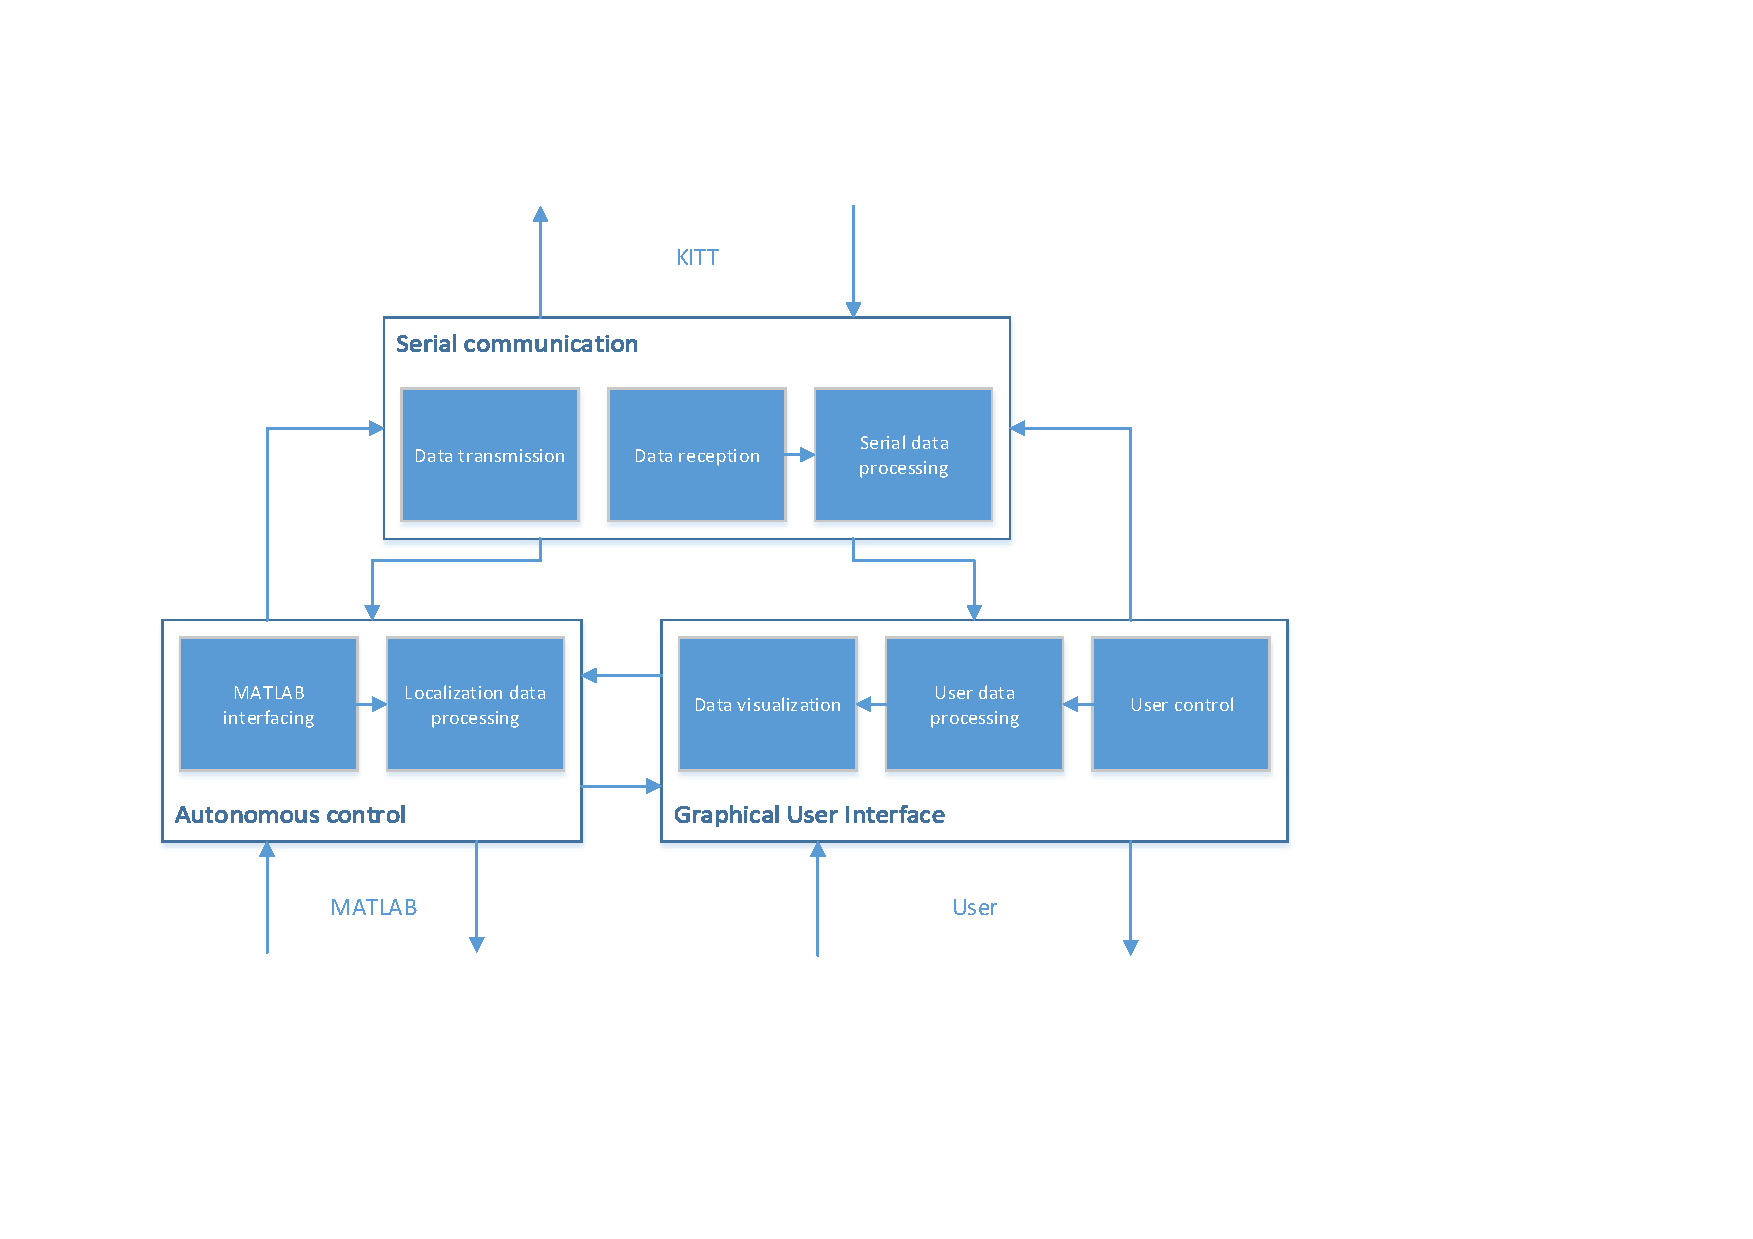
\includegraphics[width=\linewidth]{resource/overwatch-overview.pdf}
	\caption{An overview of \emph{Overwatch}, our GUI}
	\label{fig:overwatch-overview}
\end{figure}

Implementing this design in a structured way means structured programming is required, which is in our case achieved by making optimal use of the \emph{class}-structure. Also, since a lot of data needs to be accessible via the user interface, a tight link should exist between back-end (data models and processing) and front-end (the view, where data is presented to the user). In .NET, this can be achieved by making use of so-called data-bindings. These are a kind of constraints that notify the user interface when their value is being altered, so the interface is triggered to display this new data (semi-)automatically \cite{data-binding}.
Finally, the program code is set up in a pattern that is called MVVM, or Model-View-ViewModel. This means that the previously mentioned data-bindings do not directly connect the raw data from the model to the view, but an extra layer, the \emph{ViewModel}, is introduced, that prepares model data (think integer to string conversion, real-world to visualization canvas coordinate transforms, etcetera) in such a way that it can be correctly displayed by the GUI \cite{mvvm}.

\begin{figure}[H]
	\centering
	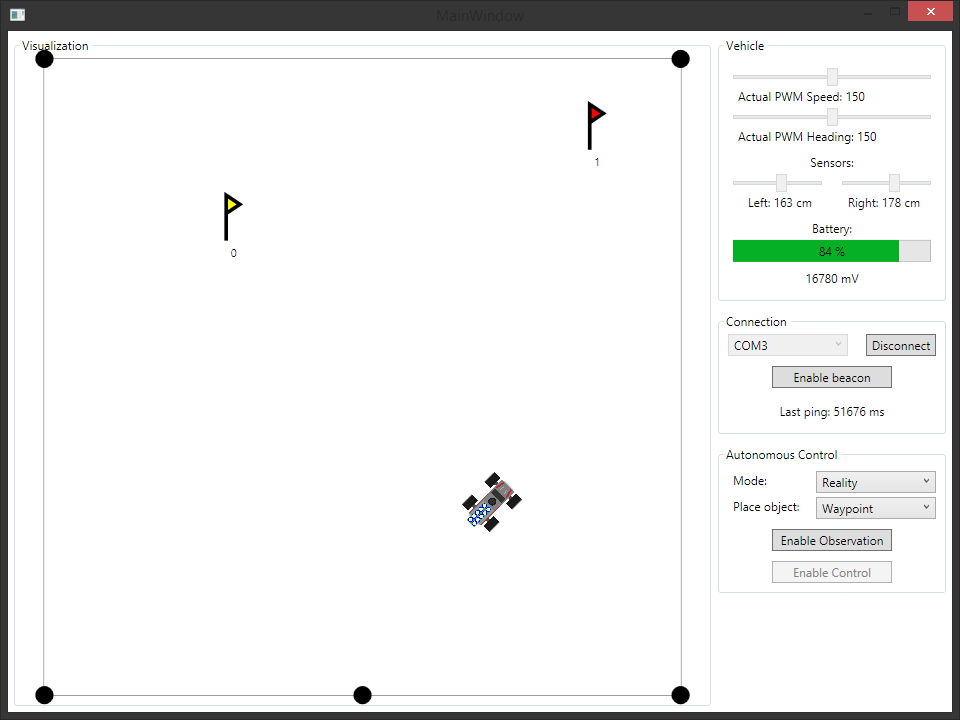
\includegraphics[width=\linewidth]{resource/overwatch-screenshot.png}
	\caption{A screenshot of Overwatch while idle}
	\label{fig:overwatch-screenshot}
\end{figure}

Figure~\ref{fig:overwatch-screenshot} gives a preview the result of our efforts. Source code of Overwatch can be found in Appendix~\ref{appsec:overwatch}. We will now discuss each of the individual subcomponents.

\section{User control}
The user needs to be able to perform some actions for enabling KITT to drive as required:

\begin{itemize}
	\item Establish the correct serial connection for communication over Bluetooth
	\item Toggle the audio beacon if needed
	\item Manipulate waypoints
	\item Toggle KITT (observation and control)
\end{itemize}

Each of these actions can be performed through Overwatch, as shown in Figure~\ref{fig:overwatch-screenshot}. Establishing a serial connection is done by selecting the correct port and clicking the button; simple toggle operations are also done via buttons; and waypoint manipulation is done on-the-fly via mouse gestures on the viewport (visualization canvas, the left part of the GUI) itself. Left clicking it creates a new waypoint on the clicked location, left clicking an existing waypoint will remove that waypoint; right clicking a waypoint will mark it as visited when not yet visited or vice-versa; and lastly, the order in which the waypoints are visited can be altered using the scroll-wheel on the waypoint that is to be reordered.

\section{Communication}
After enabling KITT, everything begins and ends with the serial interface. New data is retrieved from KITT over serial, processed and then KITT is given new commands over the same serial connection again. This process (Figure~\ref{fig:overwatch-process}) runs until KITT is disabled again.

\begin{figure}[H]
	\centering
	\begin{tikzpicture}[node distance = 2cm, auto]
	% Nodes
	\node [rectangle] (status) {Request status};
	\node [rectangle, right= of status] (autocontrol) {Perform autocontrol process};
	\node [rectangle, right= of autocontrol] (command) {Command KITT};
	\node [rectangle, below= of autocontrol, yshift= 1cm] (update) {Update GUI};
	\coordinate [left= 0.5cm of status] (c1);
	\coordinate [above left = 0.75cm and 0.5cm of status] (c2);
	\coordinate [above right= 0.75cm and 0.5 cm of command] (c3);
	\coordinate [right= 0.5cm of command] (c4);
	% Edges
	\path [line, ->] (c1) -- node {} (status);
	\path [line] (c2) -- node {} (c1);
	\path [line] (c3) -- node {} (c2);
	\path [line] (c4) -- node {} (c3);
	\path [line] (command) -- node {} (c4);
	\path [line, ->] (status) -- node {} (autocontrol);
	\path [line, ->] (autocontrol) -- node {} (command);
	\path [line, ->] (status) |- node {} (update.west);
	\path [line, ->] (autocontrol) -- node {} (update);

\end{tikzpicture}
	\caption{The process for controlling KITT, for \emph{autocontrol}, see Section~\ref{sec:gui-autocontrol}}
	\label{fig:overwatch-process}
\end{figure}

In C\#, the serial connection is handled completely asynchronously. An event is triggered as soon as data is received and other classes of the program may respond to this event, but this is not required. This asynchronous behavior means we do not have to wait for KITT to respond to any command we send it, so we can continue running the various processes in the mean time.

\section{Visualization}
Perhaps the most interesting part of Overwatch is the visualization canvas. This field is found in the left part of the GUI and occupies the majority of its space. It shows a real-time representation of the field KITT drives in, along with the placed microphones, KITT itself and all waypoints. Information about KITT's location and angle is obtained using the \texttt{MATLAB} logic previously discussed and the visualization canvas updated as soon as it becomes available. Being able to see where the localizer ``thinks'' KITT is, proved a to be a very useful feature while debugging the rest of our design and apart from that, it looks quite nice.

\section{Autonomous control}
\label{sec:gui-autocontrol}
Since we use both \texttt{MATLAB} and C\#, we need to be able to exchange data between the two, to enable autonomous control of KITT. As shown in Figure~\ref{fig:overwatch-overview}, Overwatch will receive status information from KITT, which should then be sent to \texttt{MATLAB} for processing; after which the result of this processing (PWM excitation values for driving KITT), along with localization results (for visualization), should be retrieved back from \texttt{MATLAB} by the GUI. This task, linking \texttt{MATLAB} and C\#, is executed by another subcomponent as depicted by the previously given Figure~\ref{fig:system-overview-process}. As already pointed out, the visualization canvas is automatically updated upon each relevant data change due to the autonomous control process.

\section{Future work}
With Overwatch, we delivered a robust program that meets all given requirements and is certainly better looking than anything designed in \texttt{MATLAB}. An improvement that could be implemented, however, is asynchronous handling of the \texttt{MATLAB} interface. As previously discussed, we experienced a localization delay of around \SI{2}{seconds}, due to the used ASIO drivers. During this interval, the GUI would freeze, which is suboptimal. When moving all \texttt{MATLAB} operations to a separate \emph{thread} (make it a background task), this would not occur.

\end{document}